Most probably, during your career as a programmer you have found
a seemingly simple problem that, when it increased a bit in size, you could not
get a solution for it in a reasonable amount of time. All the ideas and approaches
you had for it seemed useless and you wondered why.
And if you still have not, I guarantee that at some point you will.

This text aims to make you a more effective and knowledgeable programmer, by
providing you with the knoweledge about how to confront them. But first at all,
lets give these problems a name.

\section{Combinatorial Problems}

A \emph{combinatorial problem} consists in finding, among a finite set of
objects, one that satisfies a set of constraints. With Constraint Programming
you will be able to solve many kinds of combinatorial problems. 

Amongst combinatorial problems, the ones we are specially interested in are the
ones for which exhaustive search is not tractable. For solving these problems
we will need to identify the patterns or regularities in them and exploit these
in a clever way; to make deductions and decisions until we make our way into a
solution that satisfies all the constraints. All of this without introducing any
bug and considering all edge cases.

And as a programmer, you know that the effort in doing all of the above is not
trivial at all. Luckly for us we are not the first ones to confront these problems.

\section{What is Constraint Programming?}

The majority of programming languages were designed with the imperative
paradigm in mind. In these languages, statements describe how the program state
changes.  The work of the programmer is to devise which sequences of statements
produce the desired result. In other words, an imperative program is trying to
explain how to accomplish something to a computer.

\begin{example}
If we are given a value $x$ and we are asked to find it's square root, we might
apply the Babylonian method: (i) start with a guess $g$ (ii) improve the
guess $g$ by averaging $g$ and $x/g$ (iii) keep improving the guess $g$
until it is good enough.
%
The basic idea of the method here is that if $g$ is an overestimate to the
square root of $x$, then $x/g$ will be an underestimate. So, the average of
these two numbers will provide a better approximation.
\end{example}

In a declarative paradigm instead of focusing on \emph{how}, the programmer
should focus on describing \emph{what} the program should accomplish. 
In other words, it should describe ``what is true''.

\begin{example}
In a declarative paradigm, to find the square root of $x$ it is enough to 
state: $\sqrt{x}$ is the $y$ such that $y^2 = x$ and $y \geq 0$.
%
Note that this statement tells you what the square root is without having to
describe \emph{how} you should find the square root. 
\end{example}

The beauty of this paradigm is that it will allow us to translate a problem
statement into a solvable problem specification \emph{without} having to come
up with an imperative algorithm. 

%If we were to situate Constraint Programming in a map, it would be
%a picturesque isle between the seas of artificial intelligence, computer
%science and operations research.

Our focus here will be Constraint Programming (CP), a paradigm for solving
combinatorial problems that draws on a wide range of techniques from artificial
intelligence, computer science and operations research. 
%
Constraint Programming tools \emph{declaratively} state relations between problem
variables in the form of constraints, specifying the properties of the
solution. These constraints can take many forms, such as logical ($\neg$,$\vee$
or $\wedge$) or numerical (+, -, $*$) operators for example.
%
The set of constraints is then automatically solved by giving a value to each
variable so that the solution is consistent with the stated constraints. Do
not worry, we will give more formal and complete definitions in the future, but
for now this should suffice.

\section{Modelling}

In our setting, a \emph{model} is a translation from a natural language
description of a combinatorial problem into a computable formulation. Models
concretise the problem using a certain language that can be understood by an
application called a \emph{solver}. 
With a model, the solver will perform
analysis, inference and search on it. This process will end in solutions to the
model that can then be interpreted in terms of the original description of the
problem. Figure~\ref{fig-modelling} illustrates this process.

\begin{figure}[h]
    \label{fig-modelling}
    \centering
    \begin{tikzpicture}[node distance=2cm]
    \tikzstyle{startstop} = [rectangle, rounded corners, minimum width=3cm, minimum height=1cm,text centered, draw=black, fill=red!30]
    \tikzstyle{process} = [rectangle, minimum width=3cm, minimum height=1cm, text centered, draw=black, fill=orange!30]
    \tikzstyle{decision} = [star, text centered, draw=black, fill=green!30]
    \tikzstyle{arrow} = [thick,->,>=stealth]
    \node (start) [startstop] {Natural Language Description};
    \node (model) [process, below of=start] {Model};
    \node (solver) [decision, right of=model, xshift=2cm] {Solver};
    \node (solution) [process, right of=solver, xshift=2.5cm] {Solution to the Model};
    \node (end) [startstop, above of=solution] {Solution in Natural Language};

    \draw [arrow] (start) -- node[anchor=east] {create} (model);
    \draw [arrow] (model) -- node[anchor=north] {solve} (solver);
    \draw [arrow] (solver) -- node[anchor=north] {extract} (solution);
    \draw [arrow] (solution) -- node[anchor=east] {translate} (end);
    \end{tikzpicture}
    \caption{A high-level view of how a problem is solved}
\end{figure}

The principal task that we will be doing here is modelling: the translation of
the problem to constraints. The process will basically involve the
interpretation of the problem at hand and deciding what is the best way to
express it in a language of our choice.

\section{Tools of the Trade}

Combinatorial problem solvers can be grouped by their solving paradigm. Some
examples of those could be Constraint solvers, SAT/SMT solvers and MIP solvers.
Commonly, solvers that share a solving paradigm also share the same input
language, fostering the comparison and competition amongst them. 

As each group of solvers use their own input language, the language we use will
determine which solvers we will be able to use.
The research community has demonstrated many times that no solver is
always better than the others, as each solving technique excel in different
ways. Therefore the choice of modelling language will not only be important, but
also far from trivial.

The tool we will be using from here onwards is \emph{Savile Row}, a modelling
assistant. Savile Row provides \emph{Essence Prime}: an expressive high-level,
solver-independent language. As shown in Figure~\ref{fig-sr}, the crucial
feature of Savile Row is that it can automatically translate an Essence Prime
model to the input language of any supported solver. 

The important takeaway is that we will be able to model once, and try many
different solving approaches.  In fact, Savile Row is named after a street in
London with many bespoke tailors. The name comes from the idea of ``tailoring''
a constraint model in a variety of different ways.

\begin{figure}[h]
    \label{fig-sr}
    \centering
    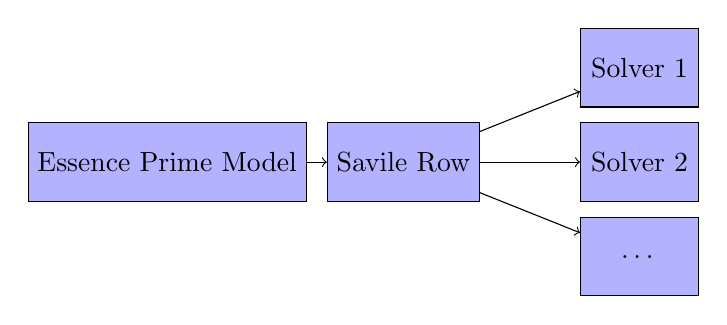
\begin{tikzpicture}[node distance=3cm]
    \tikzstyle{file} = [rectangle, minimum width=1.5cm, minimum height=1cm, draw=black, fill=blue!30]
    \node (model) [file] {Essence Prime Model};
    \node (sr) [file, right of=model] {Savile Row};
    \node (sat) [file, right of=sr] {Solver 2};
    \node (minion) [file, above of=sat, yshift=-1.8cm] {Solver 1};
    \node (other) [file, below of=sat, yshift=1.8cm] {\dots};

    \draw[->]             (model) -- (sr);
    \draw[->]             (sr) -- (sat);
    \draw[->]             (sr) -- (minion);
    \draw[->]             (sr) -- (other);
    \end{tikzpicture}
    \caption{Translation process for Savile Row models}
\end{figure}

% disconnection between the high-level mathematical concepts of modelling from
% what is available in the language of choice
